\documentclass[aspectratio=169]{beamer}

\usetheme{Madrid}
\usecolortheme{default}
\setbeamertemplate{navigation symbols}{}
\setbeamertemplate{caption}[numbered]

\usepackage[T1]{fontenc}
\usepackage{lmodern}
\usepackage{booktabs}
\usepackage{array}
\usepackage{graphicx}
\usepackage{xcolor}
\usepackage{tikz}
\usetikzlibrary{arrows.meta,positioning,shapes.geometric}

\graphicspath{{../../results/automatic_detector_gabor_depth/}
               {../../results/adjacent_bscan_experiments/single_scan_control/}
               {../../results/manual_ground_truth/}}

\definecolor{eacolor}{RGB}{230,126,34}
\definecolor{barcodecolor}{RGB}{190,55,55}
\definecolor{normalcolor}{RGB}{55,130,75}
\definecolor{mutedblue}{RGB}{48,92,145}
\newcommand{\EA}{\textcolor{eacolor}{\textbf{EA}}}
\newcommand{\Barcode}{\textcolor{barcodecolor}{\textbf{barcoding}}}
\newcommand{\Normal}{\textcolor{normalcolor}{\textbf{normal}}}

\title{Current State of the EA and Barcoding Detector}
\subtitle{What happens as an OCT scan moves through the pipeline?}
\author{Jonathan Ma}
\institute{Johns Hopkins University}
\date{August 18, 2026}

\begin{document}

\begin{frame}
    \titlepage
\end{frame}

\begin{frame}{One Scan, One Traceable Decision Path}

\begin{center}
\large
\textcolor{mutedblue}{Load the selected B-scan}
$\longrightarrow$
\textcolor{mutedblue}{Standardize the image}
$\longrightarrow$
\textcolor{mutedblue}{Measure visible patterns}

\vspace{0.35cm}

$\longrightarrow$
\textcolor{mutedblue}{Score EA and barcoding separately}
$\longrightarrow$
\textcolor{mutedblue}{Reject likely structure}

\vspace{0.35cm}

$\longrightarrow$
\textcolor{mutedblue}{Report intervals and confidence evidence}
\end{center}

\vspace{0.4cm}

The output assigns each horizontal location to \Normal, \EA, or \Barcode.
Adjacent positive columns become an interval whose location and width can be
reported. Every rejection stage records why a candidate was removed.

\vspace{0.2cm}
\small Here, ``normal'' is an operational output meaning neither phenotype was
selected; it does not certify that the retina is clinically normal.

\end{frame}

\begin{frame}{Step 1: Loading the Relevant Scan}

\begin{columns}[T]
\column{0.47\textwidth}
\begin{block}{Input}
The validation workflow opens the native HEYEX E2E volume and selects the
patient-specific B-scan number recorded in the manual annotation.
\end{block}

\column{0.47\textwidth}
\begin{block}{Anatomical reference}
The scan is loaded together with its Bruch membrane (BM) boundary. This keeps
the image and the scanner-provided retinal landmark paired throughout
processing.
\end{block}
\end{columns}

\vspace{0.5cm}

The same loader can accept a PNG with JSON metadata, but the current validation
results begin with E2E volumes so neighboring B-scans and BM metadata remain
available.

\end{frame}

\begin{frame}{Step 2: Standardizing the B-scan}

The selected preprocessing configuration is fixed across all ten cases:

\begin{table}
\centering
\small
\begin{tabular}{lll}
\toprule
\textbf{Operation} & \textbf{Selected setting} & \textbf{Result} \\
\midrule
Alignment & Flatten to BM & BM appears at a common depth \\
Region retained & 150 pixels below BM & Same anatomical depth range \\
Brightness scaling & Within-scan z-score & 0 = scan average; positive = brighter \\
Denoising & Gaussian $(1.0,0.5)$ & Mild noise reduction; stripes preserved \\
Incomplete depth & Padding allowed & Scan remains processable \\
\bottomrule
\end{tabular}
\end{table}

The detector receives a consistently aligned, approximately
$150\times512$-pixel sub-BM image.

\end{frame}

\begin{frame}{Step 3: Turning Appearance into Measurements}

At every horizontal position, the detector asks a small set of clinically
readable questions:

\begin{itemize}
    \item Is the tissue column broadly brighter than the rest of this scan?
    \item How bright are its brightest relevant pixels?
    \item Does the pattern remain aligned as it extends deeper?
    \item Does it form an organized vertical structure?
    \item Does it contain repeated bright--dark stripe texture?
    \item Is the brightness concentrated near BM, in the middle, or deeper?
\end{itemize}

Each measurement is expressed relative to the same scan. This allows the final
JSON to show which visible properties supported each interval.

\end{frame}

\begin{frame}{The Detector Architecture}

\begin{enumerate}
    \item \textbf{Candidate scores:} independent EA and barcoding models score
    every column from brightness, continuity, vertical organization, and their
    combinations.
    \item \textbf{Local context:} isolated responses are suppressed unless
    nearby columns provide compatible evidence.
    \item \textbf{Interval formation:} short gaps may be joined and very short
    detections are removed.
    \item \textbf{Structural veto:} likely vessel/structural shadows and dark
    continuous columns are excluded.
    \item \textbf{Barcoding confirmation:} the complete interval must pass
    stripe-texture and near-depth brightness checks.
    \item \textbf{Output:} remaining intervals are labeled EA or barcoding;
    all other columns are normal.
\end{enumerate}

The stages are ordered so that a structural region cannot be filled back into
a disease interval after it has been rejected.

\end{frame}

\begin{frame}{Current Architecture: Three Scores, One Final Decision}

\centering
\resizebox{0.98\textwidth}{!}{%
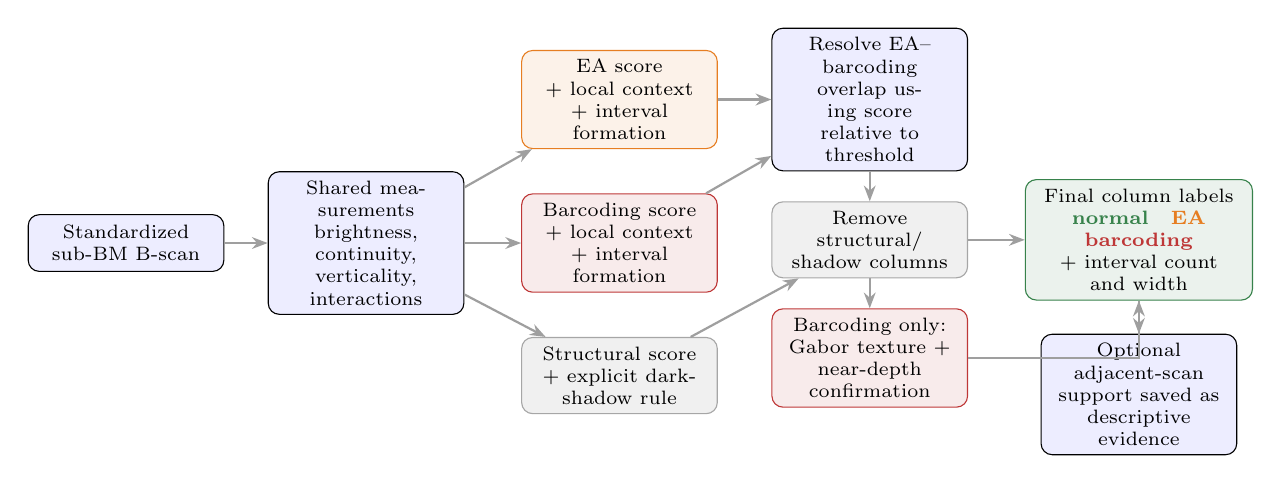
\begin{tikzpicture}[
    node distance=0.42cm and 0.55cm,
    every node/.style={font=\scriptsize,align=center},
    box/.style={draw,rounded corners,minimum height=0.72cm,
                text width=2.25cm,fill=blue!7},
    eabox/.style={box,draw=eacolor,fill=eacolor!10},
    barcodebox/.style={box,draw=barcodecolor,fill=barcodecolor!10},
    rejectbox/.style={box,draw=gray!70,fill=gray!12},
    finalbox/.style={box,draw=normalcolor,fill=normalcolor!10,
                    text width=2.65cm},
    arrow/.style={-{Stealth[length=2mm]},thick,draw=gray!75}
]
\node[box] (scan) {Standardized\\sub-BM B-scan};
\node[box,right=of scan] (features) {Shared measurements\\brightness, continuity,\\verticality, interactions};

\node[eabox,above right=0.28cm and 0.72cm of features] (ea) {EA score\\+ local context\\+ interval formation};
\node[barcodebox,right=0.72cm of features] (barcode) {Barcoding score\\+ local context\\+ interval formation};
\node[rejectbox,below right=0.28cm and 0.72cm of features] (structure) {Structural score\\+ explicit dark-\\shadow rule};

\node[box,right=0.68cm of ea] (resolve) {Resolve EA--barcoding\\overlap using score\\relative to threshold};
\node[rejectbox,below=0.38cm of resolve] (veto) {Remove structural/\\shadow columns};
\node[barcodebox,below=0.38cm of veto] (confirm) {Barcoding only:\\Gabor texture +\\near-depth confirmation};
\node[finalbox,right=0.72cm of veto] (labels) {Final column labels\\\Normal\quad \EA\quad \Barcode\\+ interval count and width};
\node[box,below=0.42cm of labels] (adjacent) {Optional adjacent-scan\\support saved as\\descriptive evidence};

\draw[arrow] (scan) -- (features);
\draw[arrow] (features) -- (ea);
\draw[arrow] (features) -- (barcode);
\draw[arrow] (features) -- (structure);
\draw[arrow] (ea) -- (resolve);
\draw[arrow] (barcode) -- (resolve);
\draw[arrow] (resolve) -- (veto);
\draw[arrow] (structure) -- (veto);
\draw[arrow] (veto) -- (confirm);
\draw[arrow] (confirm.east) -| (labels.south);
\draw[arrow] (veto) -- (labels);
\draw[arrow,dashed] (labels) -- (adjacent);
\end{tikzpicture}
}

\vspace{0.2cm}
\small The three ``models'' are interpretable linear score calculations. The
Gabor, depth, cleanup, and shadow checks are explicit rules; none is a deep
neural network.

\end{frame}

\begin{frame}{Pseudo-Algorithm for One B-scan}

\footnotesize
\begin{enumerate}
    \setlength{\itemsep}{2pt}
    \item \textbf{Measure each column:} relative brightness, brightest-pixel
    signal, depth continuity, vertical organization, Gabor texture, and
    near/middle/deep brightness.
    \item \textbf{Calculate two phenotype scores:}
    $P_{EA}(x)$ and $P_{barcode}(x)$ from the shared measurements. These are
    internal resemblance scores, not clinical probabilities.
    \item \textbf{Require spatial agreement:} blend each score with nearby
    columns, require feature votes, join short gaps, and remove short runs.
    \item \textbf{Resolve overlap:} if both phenotypes select a column, retain
    the class whose score is stronger relative to its own threshold.
    \item \textbf{Reject likely anatomy:} remove columns selected by the
    structural score or dark-shadow rule; do not fill them back in.
    \item \textbf{Confirm complete intervals:} require adequate mean and peak
    score; for barcoding, also require Gabor mean/peak and near-depth evidence.
    \item \textbf{Return the result:} label every column as normal, EA, or
    barcoding; group adjacent labels into intervals and report their widths.
    \item \textbf{Optional volume evidence:} record whether nearby B-scans
    contain a similarly located interval, without changing the selected label.
\end{enumerate}

\end{frame}

\begin{frame}{How to Read Each Detector Decision}

\scriptsize
\begin{columns}[T]
\column{0.49\textwidth}
\begin{block}{Probability score}
A number from 0 to 1 produced by combining the measured image features. It is
an internal ``how much this resembles the calibrated pattern'' score---not a
patient's probability of disease or progression.
\end{block}
\vspace{-0.08cm}

\begin{block}{Feature votes}
Three independent checks ask whether the column has above-typical
\textbf{median brightness}, \textbf{depth continuity}, and
\textbf{vertical organization}. Barcoding needs two checks to pass; EA needs
all three.
\end{block}
\vspace{-0.08cm}

\begin{block}{Local support}
The detector checks neighboring columns for near-threshold scores. A radius of
5 examines an 11-column neighborhood; a radius of 7 examines 15 columns. This
discourages isolated one-column responses.
\end{block}

\column{0.49\textwidth}
\begin{block}{Gabor mean and peak}
The Gabor measurement describes repeated vertical bright--dark texture. The
\textbf{mean} is average stripe evidence across the interval; the
\textbf{peak} is its strongest point. Values are relative to that scan: 0 is
typical, and a positive value is stronger than typical.
\end{block}
\vspace{-0.08cm}

\begin{block}{Near-depth mean}
Average relative brightness in the first 20\% of the 150-pixel region below
BM. A threshold of 0.0 means the interval must be at least as bright as the
scan-typical near-BM tissue.
\end{block}
\vspace{-0.08cm}

\begin{block}{Minimum interval}
The number of consecutive horizontal image columns required after cleanup.
These widths are pixels, not yet converted into physical distance.
\end{block}
\end{columns}

\end{frame}

\begin{frame}{Different Criteria for EA and Barcoding}

\begin{columns}[T]
\column{0.48\textwidth}
\begin{block}{\Barcode}
\begin{itemize}
    \item Internal score threshold: 0.55
    \item Minimum interval: 8 columns
    \item Local support radius: 5 columns
    \item Requires 2 of 3 feature votes
    \item Gabor mean/peak: 0.40/0.50
    \item Near-depth mean: at least 0.0
\end{itemize}
\end{block}

\column{0.48\textwidth}
\begin{block}{\EA}
\begin{itemize}
    \item Internal score threshold: 0.50
    \item Minimum interval: 12 columns
    \item Local support radius: 7 columns
    \item Requires all 3 feature votes
    \item No Gabor requirement
    \item Provisional depth gate disabled
\end{itemize}
\end{block}
\end{columns}

\vspace{0.2cm}
These are phenotype-specific decisions. The Gabor and near-depth requirements
confirm barcoding intervals only; they are not imposed on EA.

\end{frame}

\begin{frame}{How Likely Vessel or Structural Signal Is Rejected}

Two complementary checks are applied after EA/barcoding candidates form:

\begin{itemize}
    \item A structural model combines intensity, vertical organization, and
    the amount of structural edge signal. Its internal veto-score threshold is
    0.90; this is not a clinical probability.
    \item A direct dark-shadow rule identifies vertically continuous columns
    whose upper brightness is unusually low---a pattern more consistent with
    shadowing than hypertransmission.
    \item Each rejected run is expanded slightly to include its immediate
    shadow boundary.
\end{itemize}

\begin{alertblock}{Remaining challenge}
Some reproducible normal anatomy still resembles disease. It may persist into
neighboring scans and can also have strong texture and depth measurements.
\end{alertblock}

\end{frame}

\begin{frame}{What the Gabor and Depth Checks Added}

\begin{columns}[T]
\column{0.48\textwidth}
\begin{block}{Stripe-texture evidence}
Three pattern widths---4, 8, and 16 pixels---are examined. A candidate must
show repeated vertical bright--dark variation across the interval, rather than
a single bright column.
\end{block}

\column{0.48\textwidth}
\begin{block}{Depth evidence}
The sub-BM image is summarized in near (0--20\%), middle (20--50\%), and deep
(50--100\%) bands. The selected barcoding rule requires at least average
near-band brightness.
\end{block}
\end{columns}

\vspace{0.4cm}

On the ten-scan development set, these checks preserved all 424 barcoding
columns that V3 correctly overlapped with the manual labels, while reducing
incorrectly marked columns from 302 to 95.

\end{frame}

\begin{frame}{Adjacent B-scans: Confidence, Not a Mandatory Veto}

For each interval, the detector checks two neighboring B-scans on either side
for another detector interval assigned the same EA/barcoding class at a similar
horizontal location.

\begin{center}
\begin{tabular}{ll}
\toprule
\textbf{Observed support} & \textbf{Suggested interpretation} \\
\midrule
Both sides & Higher volume-consistency confidence \\
At least one neighbor & Moderate volume-consistency confidence \\
No neighboring match & Lower confidence; retain for now \\
\bottomrule
\end{tabular}
\end{center}

Mandatory adjacency improved precision but removed manually annotated
intervals. Persistent vessel/anatomical patterns also survived it. Adjacent
support is therefore saved as descriptive evidence rather than used as either
a calibrated probability or a selected final gate.

\end{frame}

\begin{frame}{Validation Set and How to Read the Scores}

Ten selected B-scans were manually annotated by the research team: five from
the fast-progressing group and five from the slow-progressing group. These are
not clinician-adjudicated labels. Uncertain and vessel/structural areas are
excluded from scoring.

\begin{columns}[T]
\column{0.31\textwidth}
\begin{block}{Precision}
Of the columns marked by the detector, how many were annotated as that
phenotype?
\end{block}
\column{0.31\textwidth}
\begin{block}{Recall}
Of the manually marked phenotype, how much did the detector recover?
\end{block}
\column{0.31\textwidth}
\begin{block}{Dice}
A combined measure of overlap, false alarms, and misses. One is perfect.
\end{block}
\end{columns}

\vspace{0.3cm}
\textbf{Important:} these ten scans also informed parameter selection. The
results describe current development performance, not clinical validation.

\end{frame}

\begin{frame}{Current Best Aggregate Results}

\begin{table}
\centering
\begin{tabular}{llccc}
\toprule
\textbf{Class} & \textbf{Configuration} & \textbf{Precision} &
\textbf{Recall} & \textbf{Dice} \\
\midrule
Barcoding & V2 & 0.526 & 0.506 & 0.516 \\
Barcoding & Contextual V3 & 0.584 & 0.520 & 0.550 \\
Barcoding & Initial Gabor & 0.777 & 0.458 & 0.576 \\
Barcoding & \textbf{Gabor + depth} & \textbf{0.817} & \textbf{0.520} & \textbf{0.636} \\
\midrule
EA & V2 & 0.369 & \textbf{0.739} & 0.492 \\
EA & \textbf{V3 alone} & \textbf{0.475} & 0.699 & \textbf{0.566} \\
EA & Selected 0818 combined output & 0.462 & 0.699 & 0.557 \\
\bottomrule
\end{tabular}
\end{table}

The selected 0818 pipeline uses Gabor + depth for barcoding and no experimental
EA depth gate. Its combined EA output is slightly lower than the best EA-only
V3 run because resolving the two classes changes seven columns in one scan.

\end{frame}

\begin{frame}{What Worked---and What Did Not}

\begin{columns}[T]
\column{0.48\textwidth}
\begin{block}{Useful additions}
\begin{itemize}
    \item Separate EA/barcoding calibration
    \item Local spatial support
    \item Structural and dark-shadow vetoes
    \item Multi-scale stripe texture
    \item Near-depth barcoding evidence
\end{itemize}
\end{block}

\column{0.48\textwidth}
\begin{block}{Not selected}
\begin{itemize}
    \item Additional learned normal model
    \item Mandatory adjacent support
    \item Bilateral volume veto
    \item Conservative hybrid rejection
    \item Balanced hybrid rejection
\end{itemize}
\end{block}
\end{columns}

\vspace{0.25cm}
The hybrid rules combined absent neighbor support, short width, and weak
texture/depth/internal scores. They removed correctly overlapping columns
faster than incorrect columns; the control retained the best Dice.

\end{frame}

\begin{frame}{Strong Barcoding Case: Fast 49, B-scan 33}

\begin{columns}[T,onlytextwidth]
\column{0.49\textwidth}
\centering
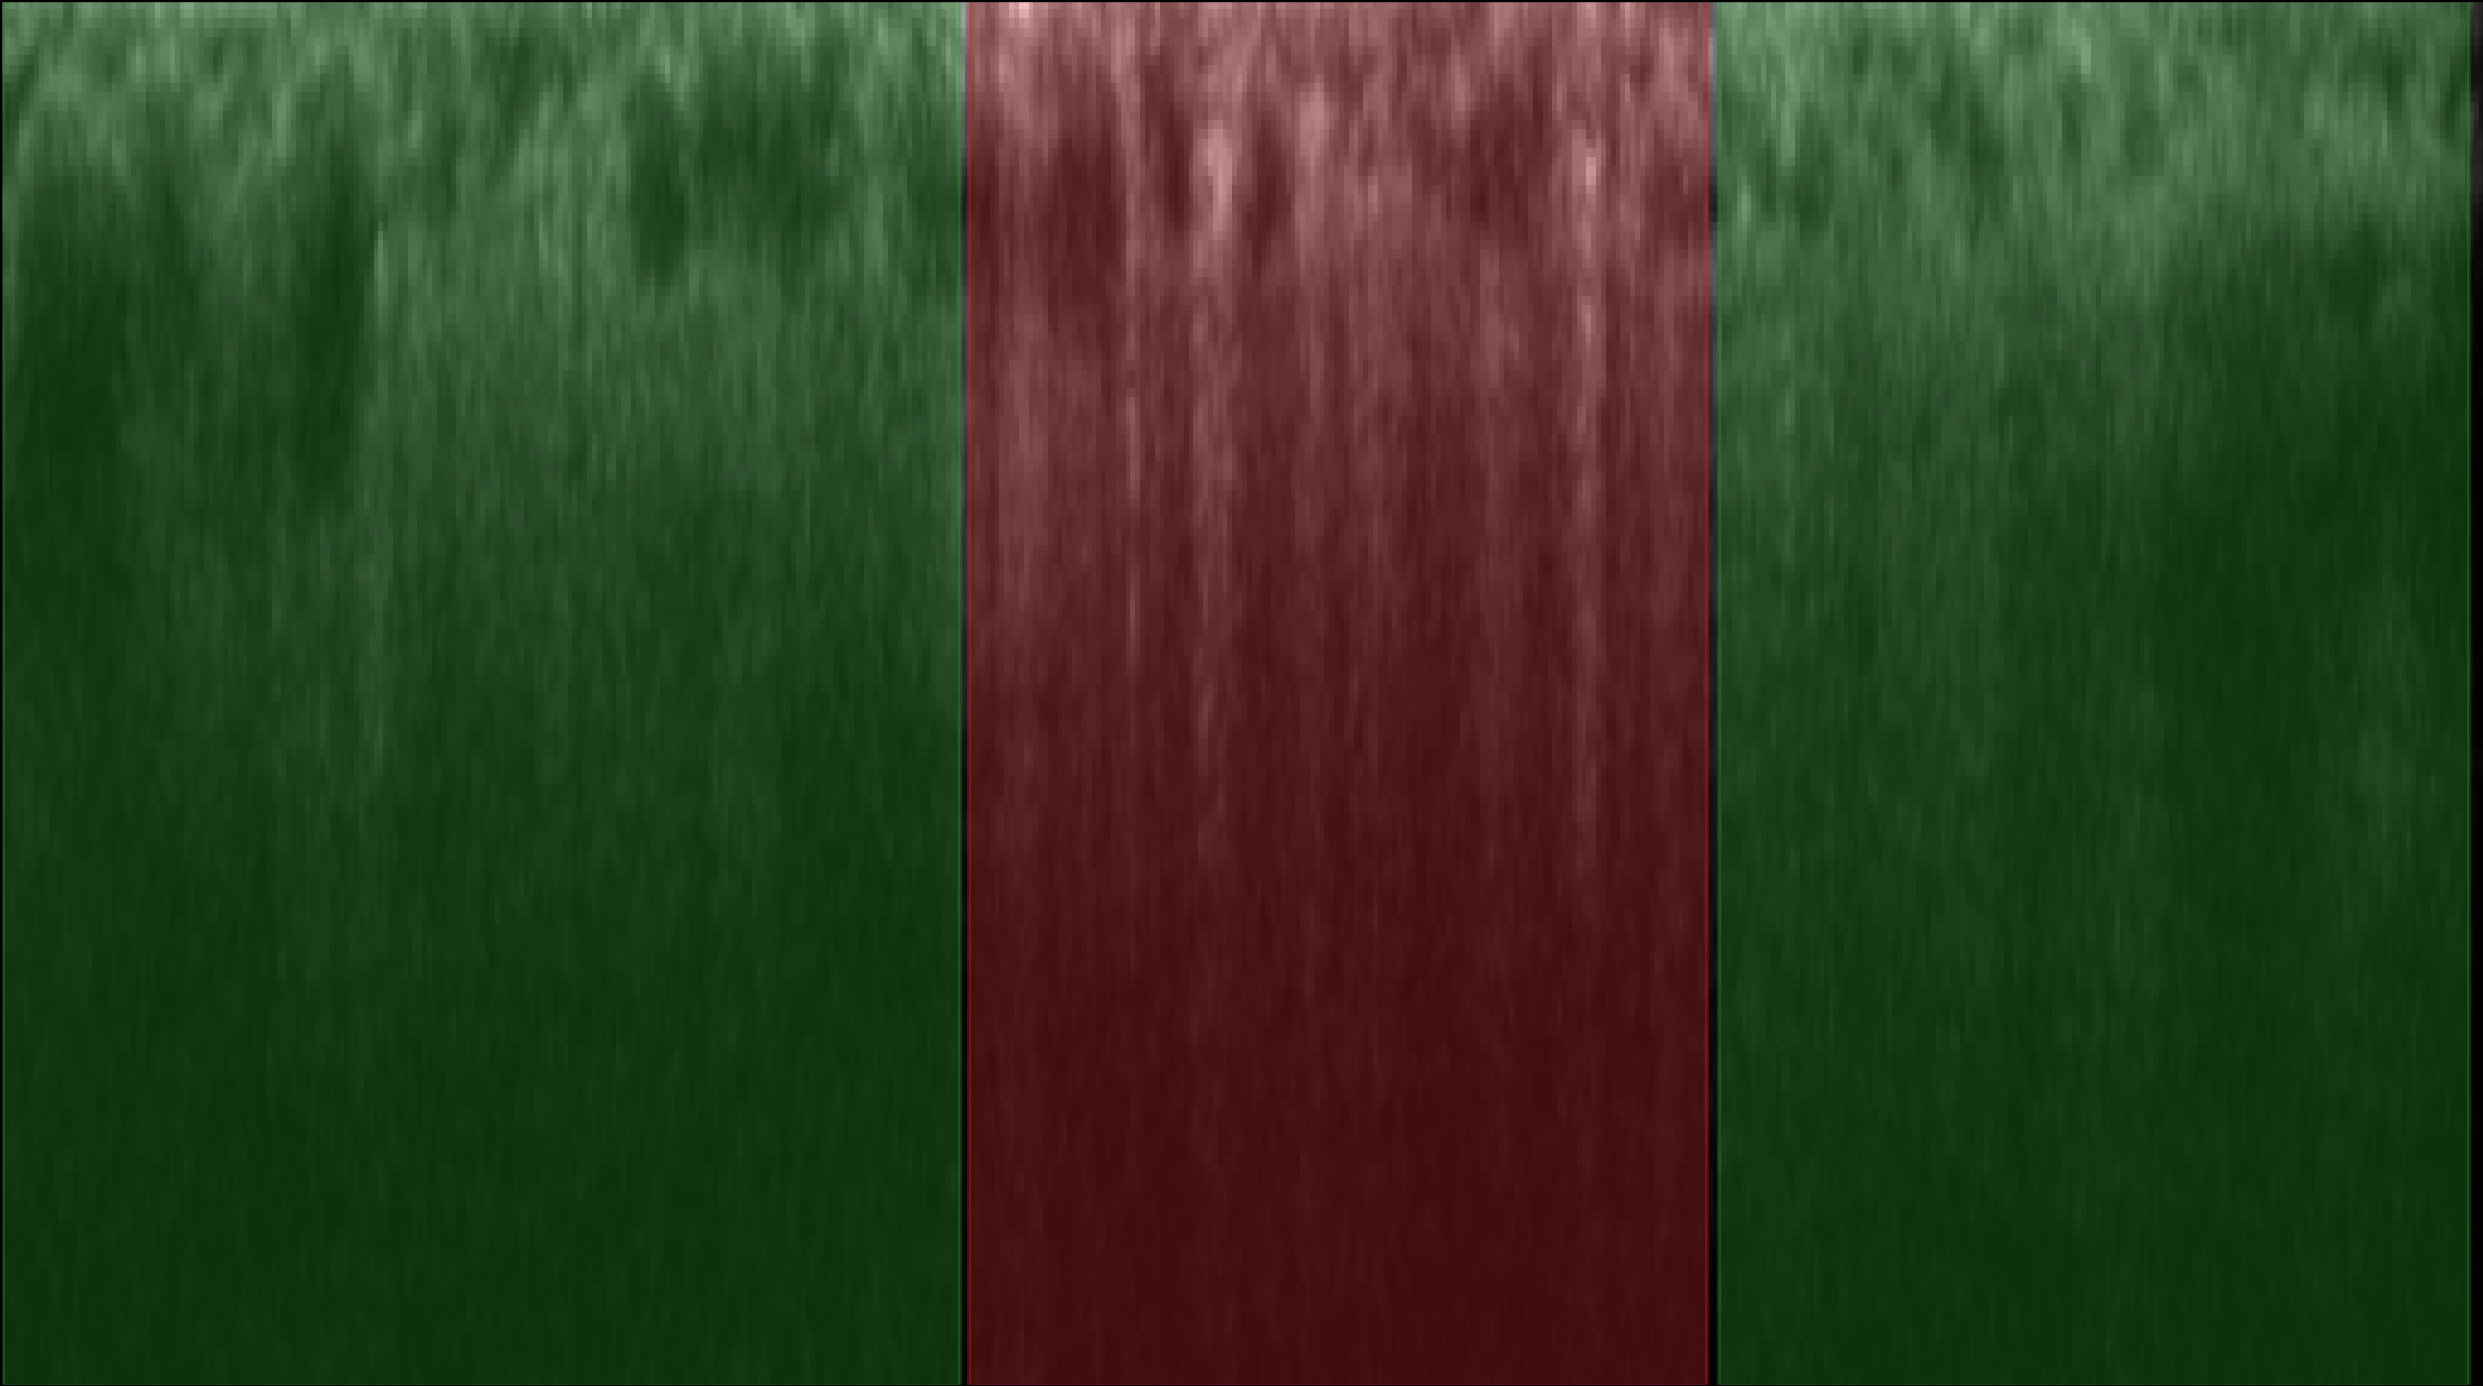
\includegraphics[width=\linewidth,height=0.28\textheight]{fast_49_bscan_033_ground_truth.png}

\small Manual annotation

\column{0.49\textwidth}
\centering

\includegraphics[width=\linewidth,height=0.28\textheight]{fast_49_bscan_033_automatic.png}

\small Automatic output
\end{columns}

\vspace{0.2cm}
\centering
\Barcode: precision 0.93, recall 0.78, Dice 0.85.

The detector localizes the major barcoding regions closely, with relatively
little additional marked tissue.

\end{frame}

\begin{frame}{Strong EA Case: Slow 47, B-scan 31}

\begin{columns}[T,onlytextwidth]
\column{0.49\textwidth}
\centering
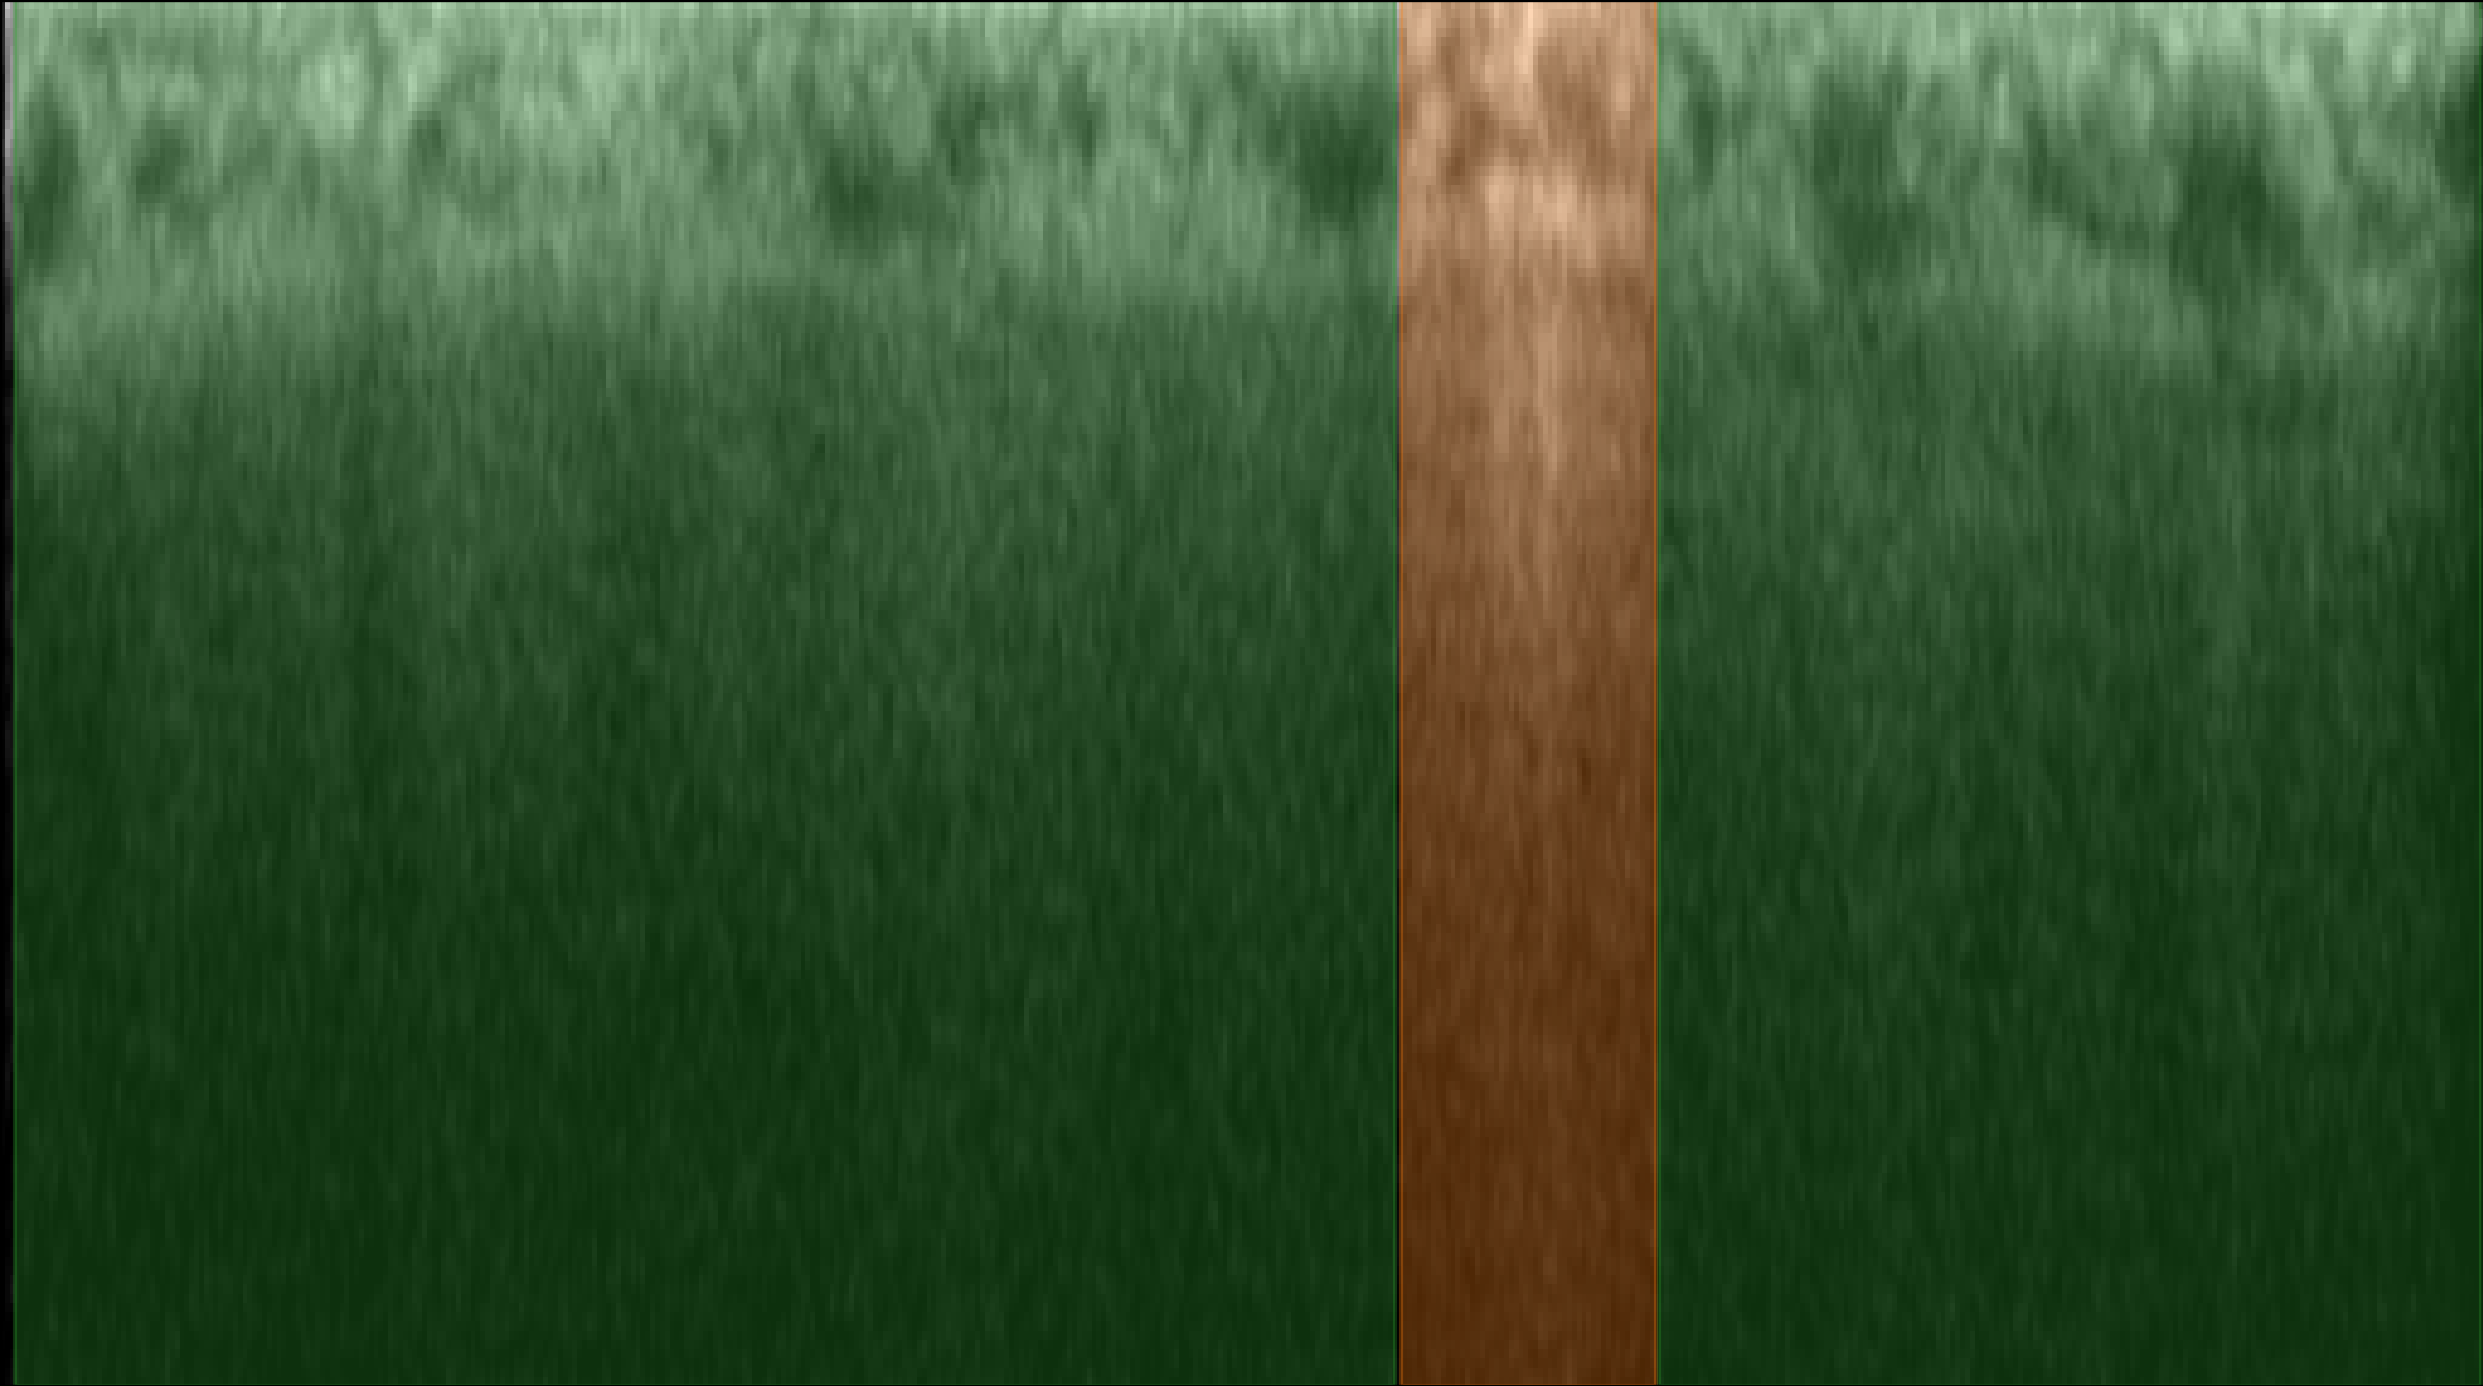
\includegraphics[width=\linewidth,height=0.28\textheight]{slow_47_bscan_031_ground_truth.png}

\small Manual annotation

\column{0.49\textwidth}
\centering

\includegraphics[width=\linewidth,height=0.28\textheight]{slow_47_bscan_031_automatic.png}

\small Automatic output
\end{columns}

\vspace{0.2cm}
\centering
\EA: precision 1.00, recall 0.91, Dice 0.95.

The automatic interval nearly reproduces the location and extent of the
manually marked EA region.

\end{frame}

\begin{frame}{Weak Barcoding Case: Fast 41, B-scan 59}

\begin{columns}[T,onlytextwidth]
\column{0.49\textwidth}
\centering
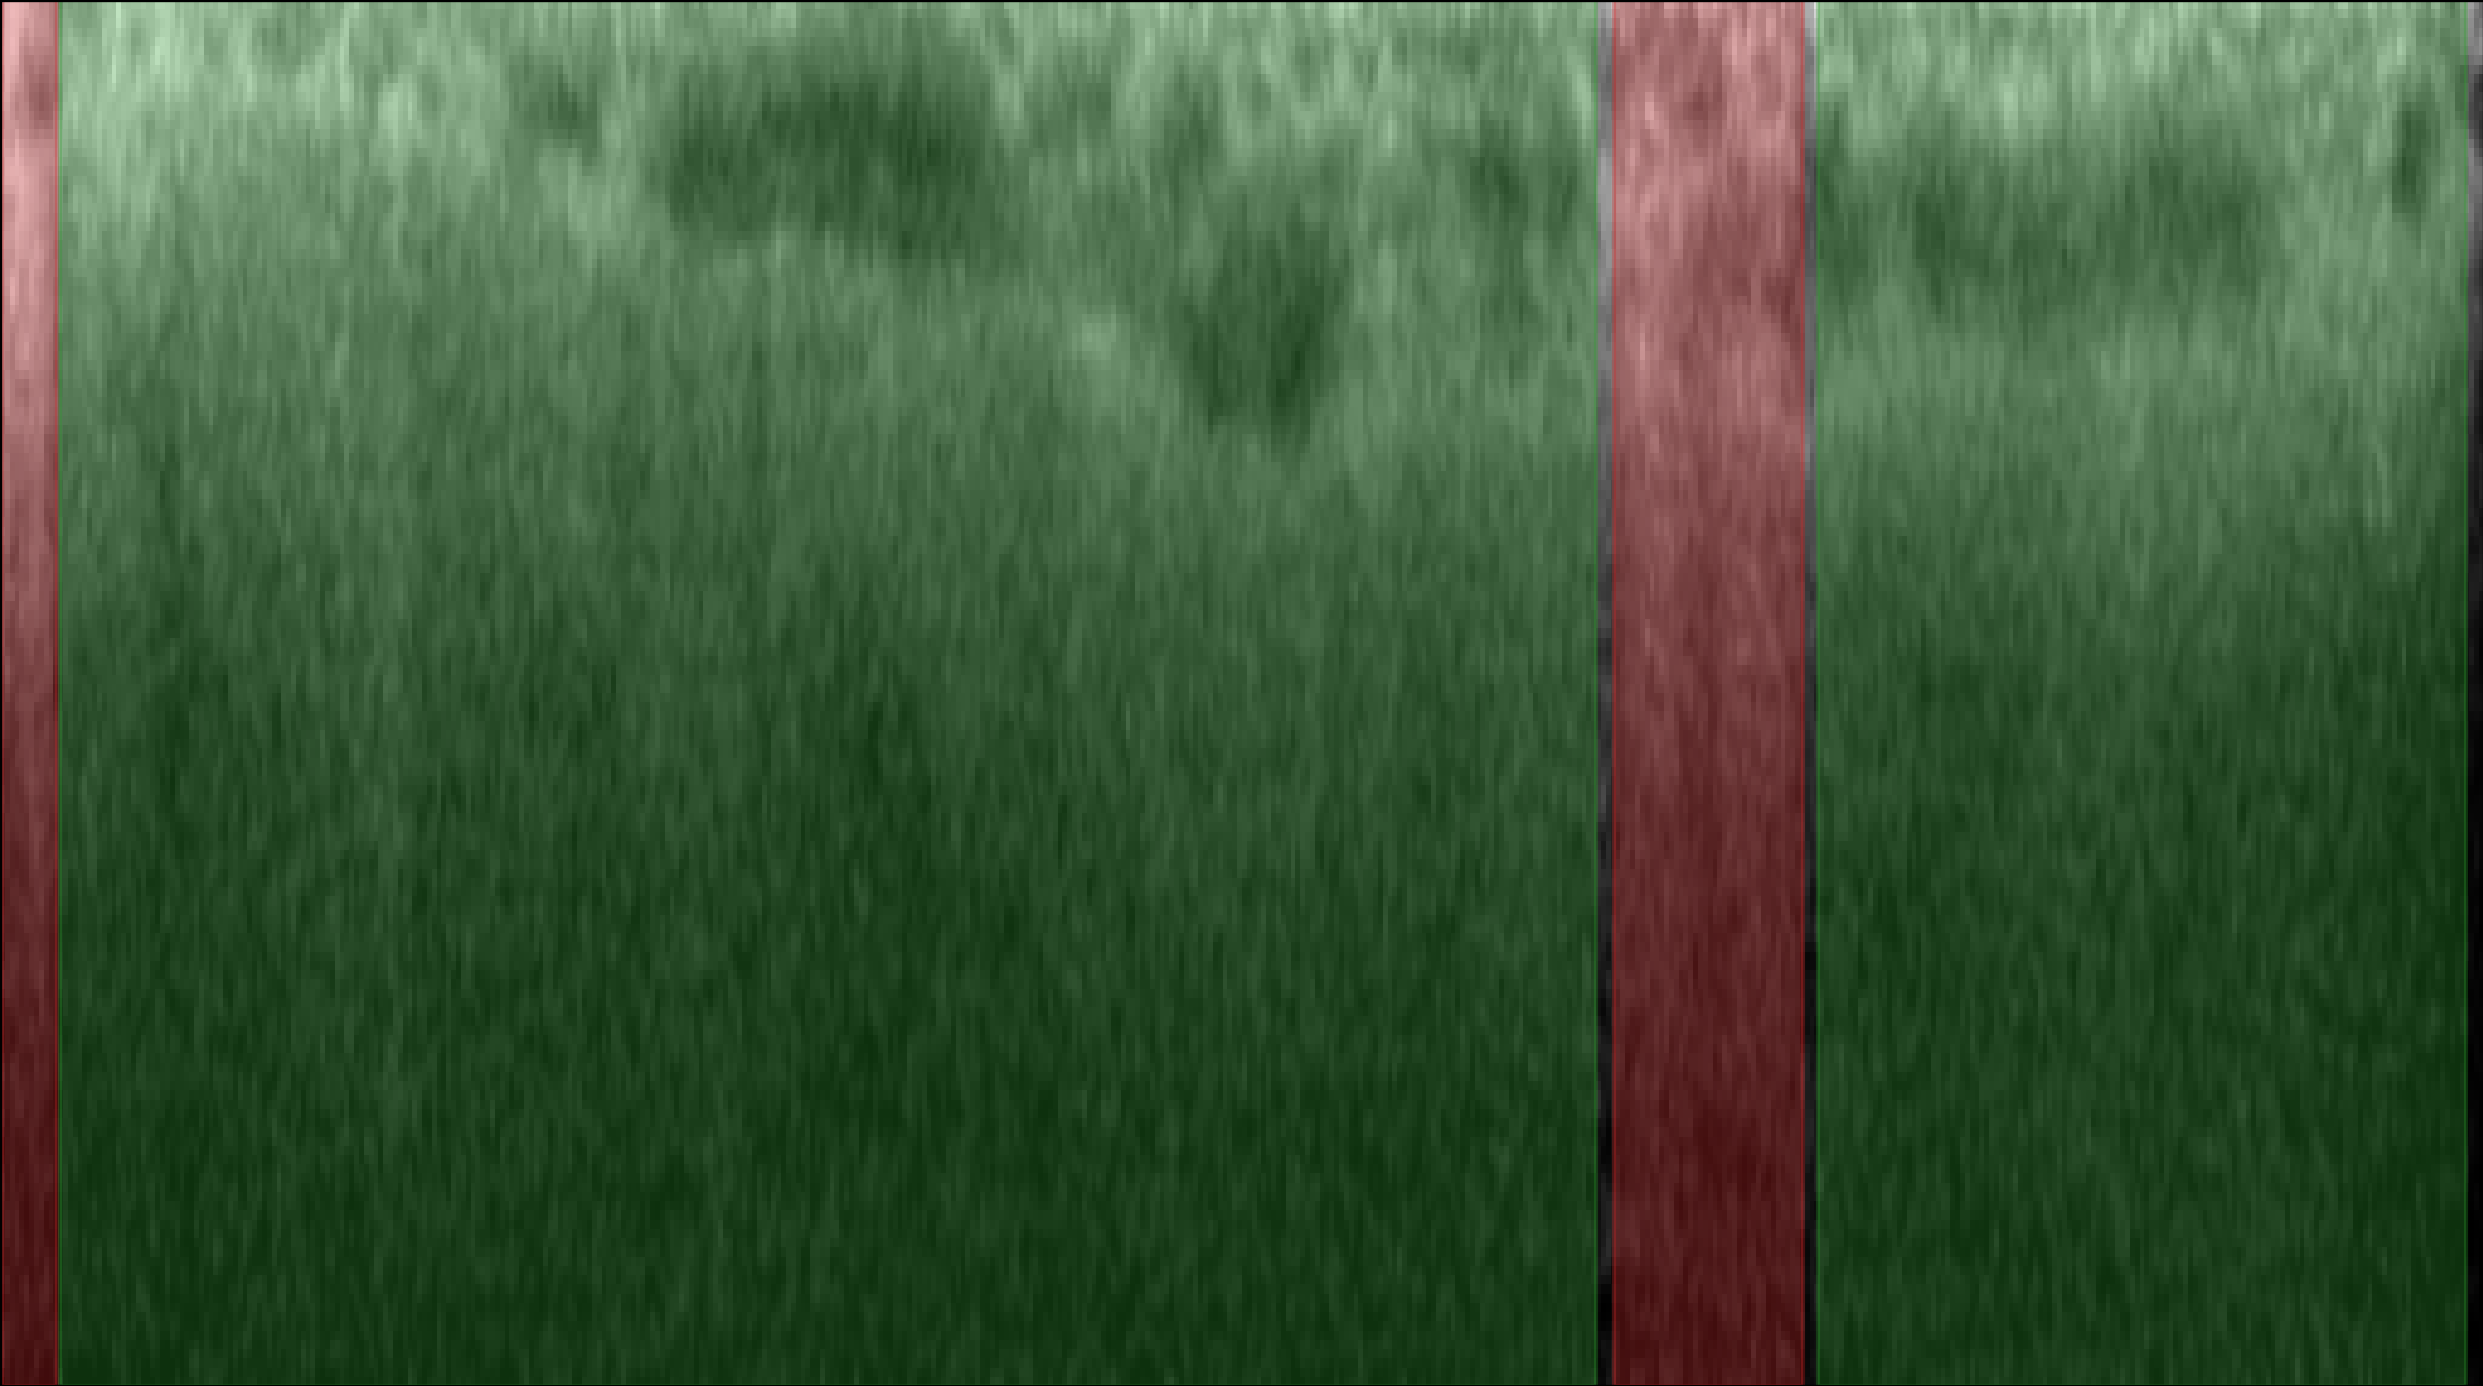
\includegraphics[width=\linewidth,height=0.28\textheight]{fast_41_bscan_059_ground_truth.png}

\small Manual annotation

\column{0.49\textwidth}
\centering

\includegraphics[width=\linewidth,height=0.28\textheight]{fast_41_bscan_059_automatic.png}

\small Automatic output
\end{columns}

\vspace{0.15cm}
\centering
\Barcode: precision 0.06, recall 0.06, Dice 0.06.

Repeatable structural patterns survive the current veto and account for 49 of
the 95 remaining false-positive barcoding columns across the development set.

\end{frame}

\begin{frame}{Another Weak Case: Fast 12, B-scan 38}

\begin{columns}[T,onlytextwidth]
\column{0.49\textwidth}
\centering
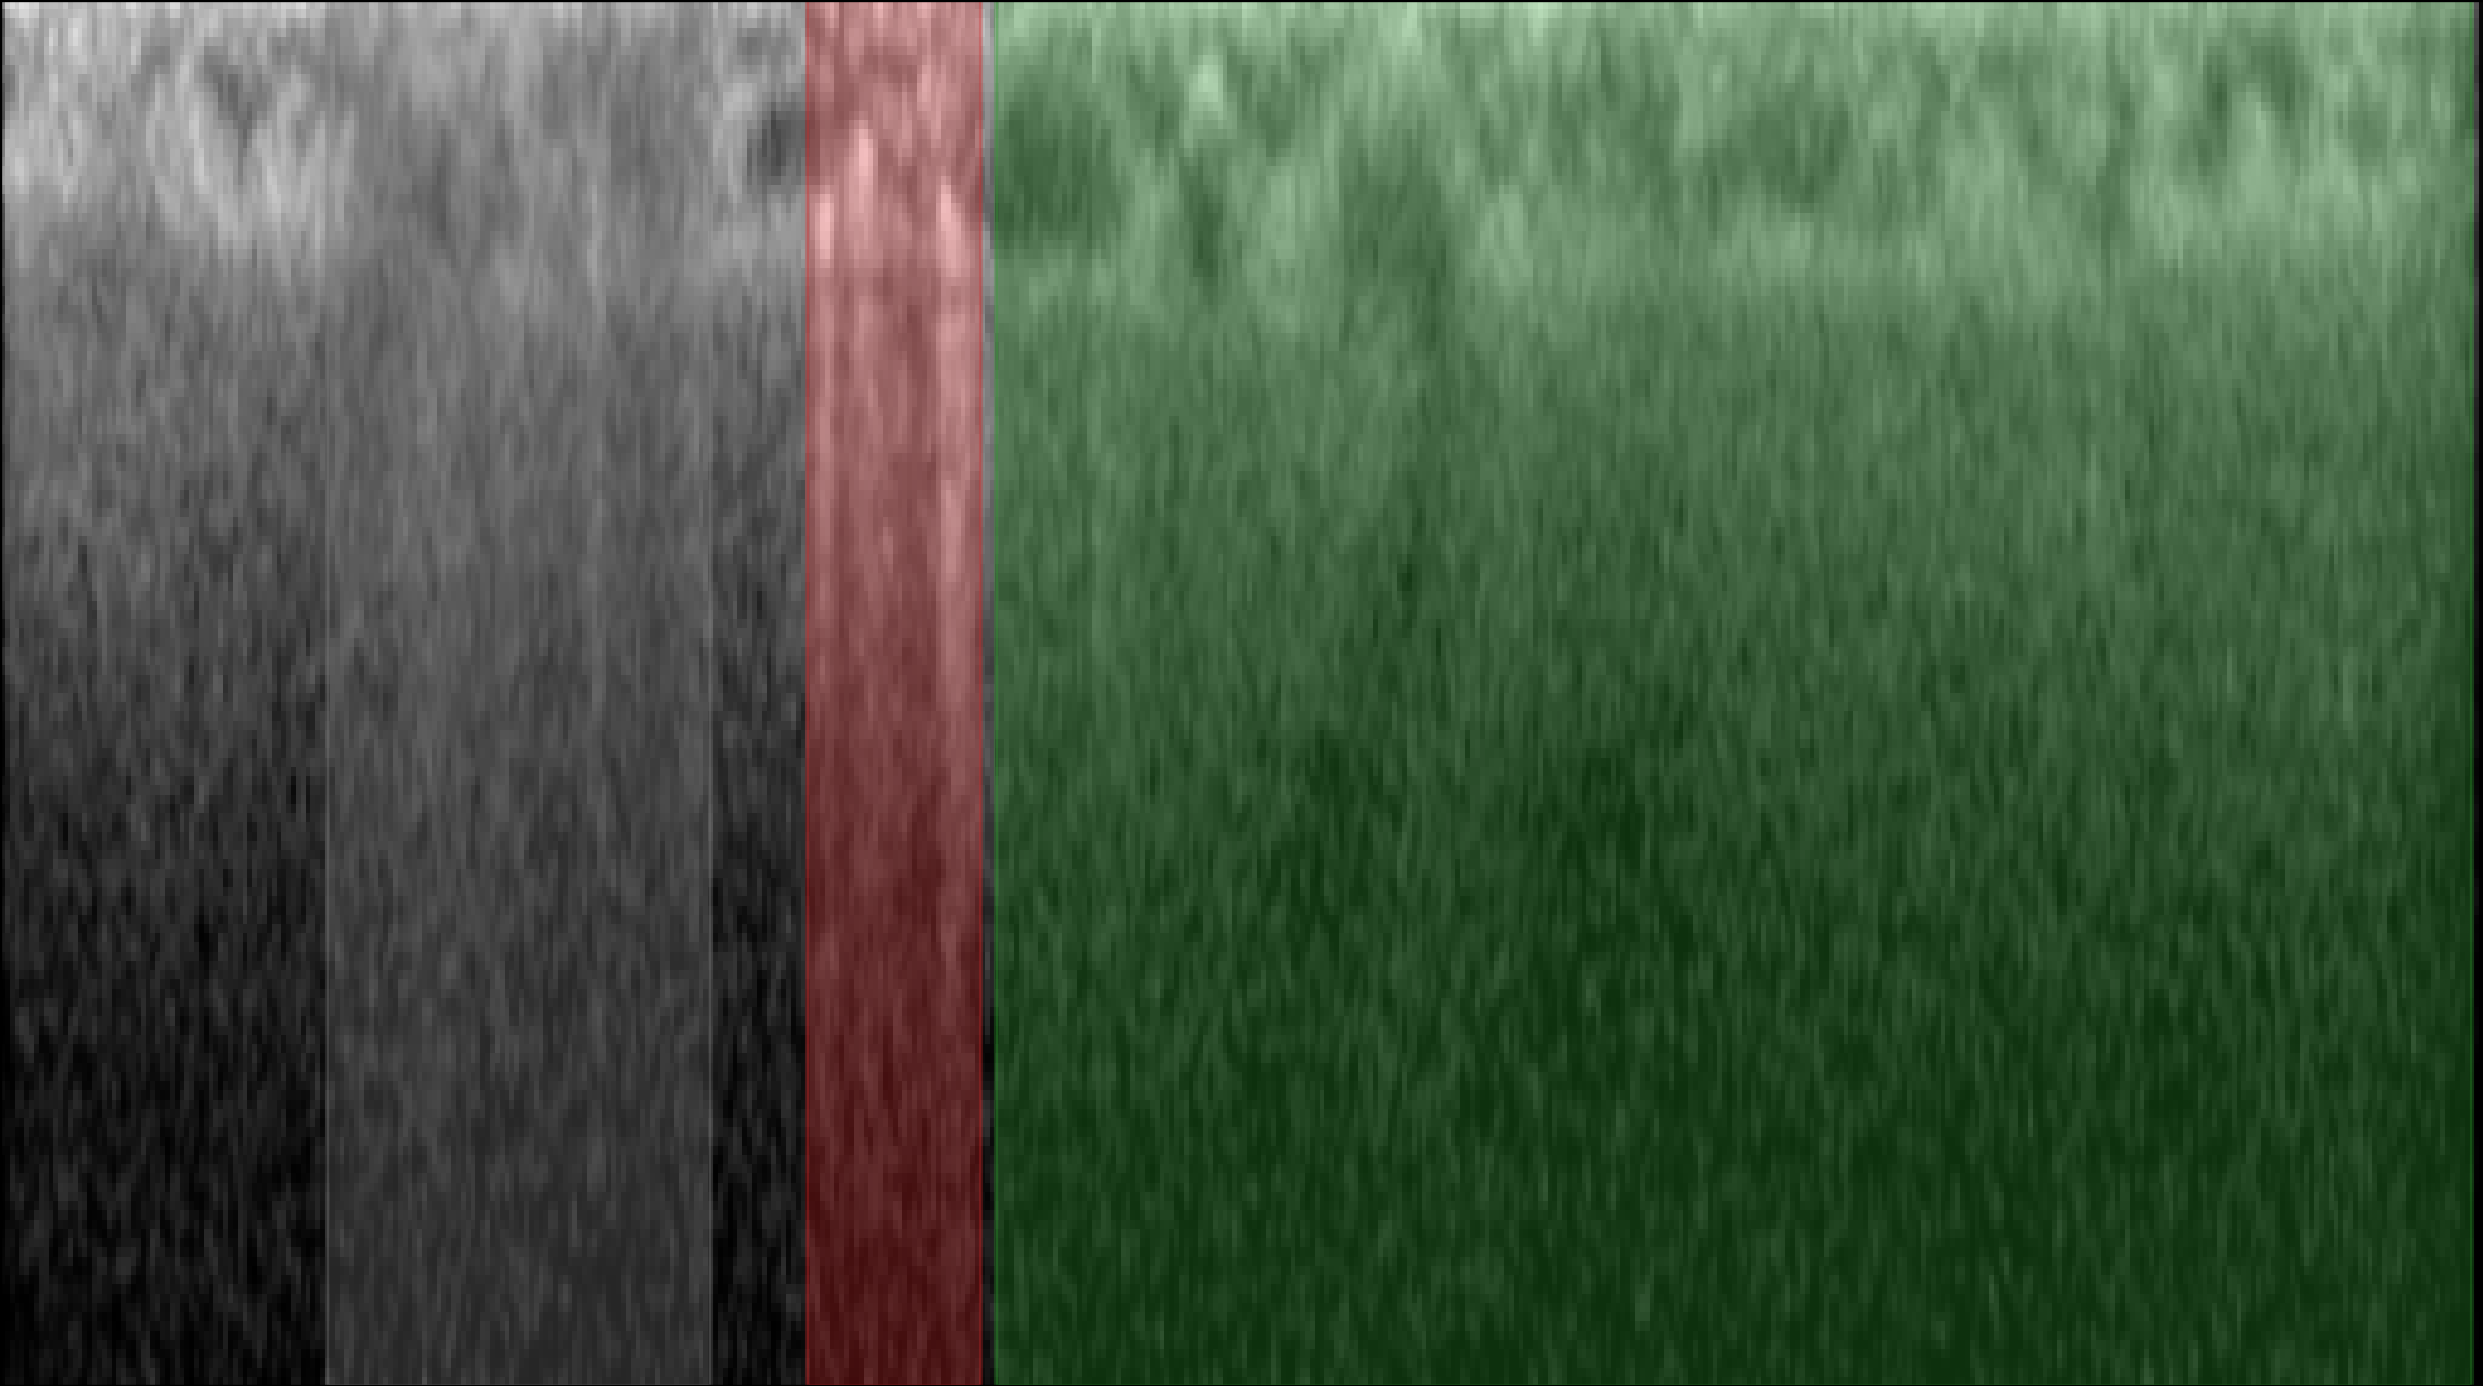
\includegraphics[width=\linewidth,height=0.28\textheight]{fast_12_bscan_038_ground_truth.png}

\small Manual annotation

\column{0.49\textwidth}
\centering

\includegraphics[width=\linewidth,height=0.28\textheight]{fast_12_bscan_038_automatic.png}

\small Automatic output
\end{columns}

\vspace{0.15cm}
\centering
\Barcode Dice 0.44; an EA interval absent from the manual annotation is also
marked.

This case illustrates both incomplete recovery of manually marked barcoding
and possible confusion between a bright structural region and EA.

\end{frame}

\begin{frame}{Why the Hybrid and Volume Rules Were Not Selected}

\begin{table}
\centering
\small
\begin{tabular}{lccc}
\toprule
\textbf{Barcoding rule} & \textbf{Precision} & \textbf{Recall} & \textbf{Dice} \\
\midrule
\textbf{Single-scan control} & 0.817 & \textbf{0.520} & \textbf{0.636} \\
Any one neighbor & 0.872 & 0.479 & 0.618 \\
Bilateral neighbors & \textbf{0.982} & 0.336 & 0.501 \\
Hybrid conservative & 0.810 & 0.497 & 0.616 \\
Hybrid balanced & 0.835 & 0.479 & 0.608 \\
\bottomrule
\end{tabular}
\end{table}

The conservative hybrid removed 19 true columns and no false columns. The
balanced version removed 18 false columns but also 34 true columns. Current
texture, depth, internal score, and adjacency evidence cannot reliably
distinguish every structural false positive from a manually marked short
interval.

\end{frame}

\begin{frame}{Current Output for Each Scan}

For every processed B-scan, the pipeline now produces:

\begin{itemize}
    \item a PNG overlay showing EA and barcoding intervals;
    \item the number of intervals for each phenotype;
    \item each interval's start, end, and width in image pixels (not microns);
    \item EA and barcoding internal scores and contextual decisions;
    \item texture and near/middle/deep brightness evidence;
    \item structural and dark-shadow exclusions;
    \item matching intervals in adjacent scans and a volume-support count.
\end{itemize}

This provides a trace from the final highlighted interval back to the evidence
that allowed it to remain.

\end{frame}

\begin{frame}{Future Direction}

\begin{enumerate}
    \item \textbf{Add genuinely different structural evidence.} Compare the
    vertical brightness profile inside a candidate with neighboring normal
    tissue. The testable hypothesis is that vessel shadowing darkens deeper
    signal, whereas hypertransmission brightens it.
    \item \textbf{Keep volume support as confidence.} Report bilateral,
    one-neighbor, or unsupported status without automatically deleting a
    lesion.
    \item \textbf{Expand independent annotation.} Additional patients and
    clinician review are more valuable now than further tuning on the same ten
    scans.
    \item \textbf{Lock and test parameters.} Evaluate the selected settings on
    untouched subjects before interpreting them as reliable biomarkers.
\end{enumerate}

\begin{block}{Current selected state}
One combined configuration: contextual V3 for both classes, with Gabor and
near-depth confirmation applied only to barcoding. Adjacent evidence is
explanatory, not a hard rejection rule.
\end{block}

\end{frame}

\begin{frame}{Take-Home Message}

\begin{itemize}
    \item The scan moves through a transparent sequence of anatomical
    alignment, visible feature measurement, phenotype-specific scoring, and
    structural rejection.
    \item Gabor texture plus near-depth evidence produced the largest barcoding
    improvement: precision 0.817 and Dice 0.636.
    \item In the selected combined 0818 output, EA has precision 0.462, recall
    0.699, and Dice 0.557; the best EA-only V3 run reached Dice 0.566.
    \item More aggressive volume and hybrid rejection increased selectivity
    but removed too much real disease signal.
    \item The main limitation is distinguishing persistent normal/vascular
    anatomy from true pathology with only ten non-clinician-adjudicated scans.
\end{itemize}

\vspace{0.3cm}
\centering
\large The next improvement should add new anatomical evidence, not merely
recombine the current scores.

\end{frame}

\end{document}
